\documentclass[article,moreauthors,pdftex,10pt,a4paper]{ssrn} 
\usepackage{algpseudocode}
%\usepackage{algorithm}
\usepackage[boxruled, lined, vlined]{algorithm2e}
\usepackage{multicol}
\usepackage{placeins}
\usepackage[title]{appendix}
\usepackage{bm}
\usepackage{subcaption}
\usepackage{lscape}
\usepackage{longtable,hhline}
\usepackage{pifont}
\usepackage{bbm}
\allowdisplaybreaks

\newcommand{\chighlight}[1]{%
\colorbox{red!50}{$\displaystyle#1$}}
\DeclareMathSizes{10}{9}{7}{6}
\DeclareMathOperator*{\tr}{\text{Tr}}
\DeclareMathOperator*{\myvec}{\text{vec}}
\DeclareMathOperator*{\diag}{diag}
\DeclareMathOperator*{\argmin}{argmin}
\DeclareMathOperator*{\argmax}{argmax}
\usepackage{colortbl}%
\newcommand{\myrowcolour}{\rowcolor[gray]{0.925}}


\graphicspath{{figs/} }

%=================================================================
\firstpage{1} 
\makeatletter 
\setcounter{page}{\@firstpage} 
\makeatother 

%% TODO: add date, make smaller names of authors, fix correspondence with cross and corresponding aurthor.
%------------------------------------------------------------------
% The following line should be uncommented if the LaTeX file is uploaded to arXiv.org
%\pdfoutput=1

%=================================================================
% Add packages and commands here. The following packages are loaded in our class file: fontenc, calc, indentfirst, fancyhdr, graphicx, lastpage, ifthen, lineno, float, amsmath, setspace, enumitem, mathpazo, booktabs, titlesec, etoolbox, amsthm, hyphenat, natbib, hyperref, footmisc, geometry, caption, url, mdframed, tabto, soul, multirow, microtype, tikz

%=================================================================
%% Please use the following mathematics environments: Theorem, Lemma, Corollary, Proposition, Characterization, Property, Problem, Example, ExamplesandDefinitions, Hypomanuscript, Remark, Definition
%% For proofs, please use the proof environment (the amsthm package is loaded by the MDPI class).
\graphicspath{{figs/} }
%=================================================================
% Full title of the paper (Capitalized)
\Title{Notes: Empirical Mode Decomposition \& Gaussian Processes}

% Author Orchid ID: enter ID or remove command
%\newcommand{\orcidauthorA}{0000-0000-000-000X} % Add \orcidA{} behind the author's name
%\newcommand{\orcidauthorB}{0000-0000-000-000X} % Add \orcidB{} behind the author's name

% Authors, for the paper (add full first names)
\Author{}

% Authors, for metadata in PDF
\AuthorNames{}

\address{% 
}

% Contact information of the corresponding author
\corres{}



\begin{document}

\begin{abstract}
Extension 1, Estimation: Treat each IMF as a separate Gaussian process and then represent the signal using multi-kernel representation of the Gaussian Process. \\
Extension 2, Forecasting: GP representation does not ensures itself that the predicted function from a given Gaussian process is IMF , that is, it satisfies (I1)-(I2). Therefore, we  explore the formulation of IMFs as an analogue of Brownian Bridge.
\end{abstract}
\tableofcontents



\section{Gaussian Processes and EMD: IMFs as Gaussian Processes with non-stationary kernels}
We treat each IMF as a separate Gaussian process and then represent the signal using multi-kernel representation of the Gaussian Process.

\subsection{The Stochastic Representation by Gaussian Processes}
Let $s(t)$ for $t\in [0,\infty]$ be a continuous signal which is observed on discrete grid of points in the interval $[0,T]$. We consider not so uncommon situation, when the observed values of $s(t)$ are perturbed by some noise component. The perturbation of the true signal can be either deterministic or stochastic. The deterministic noise might be a results of  a chaotic 


 and therefore the process which we observe is in fact
\begin{equation}\label{eq:signal_noisy_y}
y(t) = s(t) + \epsilon, \text{ for } \epsilon \in \mathcal{N}(0, \sigma^2).
\end{equation}
Therefore, our observation set consist of the pairs $\big\{t_n,y_n\big\}$ where $y_n = y(t_n)$ for $t_n \in [0,T]$. Let us remark that for the same

 the realisations of the continuous signal $s(t)$ on the discrete sent of points. W


Let $x(t)$ be a continuous real-valued signal which is an approximation of the signal $s(t)$ based on its observed values. Therefore, $x(t)$ is  

and let us define its EMD decomposition into $K$ intrinsic mode functions (IMFs) given by 
\begin{equation}\label{eq:model_x_EMD}
x(t) = \sum_{m = 1}^M c_m(t) + r_m(t) = \sum_{m = 1}^M \text{Re}\Big\{ A_m(t)  e^{i \theta_m(t)} \Big\} + r_M(t).
\end{equation}
where $r_k$ is a tendency which does not have much of oscillation and therefore characterize the low frequency tend of $x(t)$. In order to reconstruct the stochastic representation of $x(t)$ given by EMD decomposition we assume that each of the IMFs functions, $c_m(t)$, is a Gaussian process 
\begin{equation}\label{eq:model_IMF_GP_k}
c_k(t) \sim \mathcal{GP} \Big(0, k_m(t,t')\Big), 
\end{equation}
where $k_m(t,t')$ is a positive definite covariance kernel which is parametrized by a set of parameters $\Psi_m$.   The component $r_M(t)$ can be modelled as a Gaussian process itself or one can assume that $x(t)$ is Gaussian Process conditioned on $r_M(t)$, that is
\begin{equation}\label{eq:xt_conditional_rep}
x(t) | r_M(t) \sim \mathcal{GP} \Big(r_M(t),  k(t,t')  \Big).
\end{equation}
These two approaches provide an unconditional and conditional stochastic representation of $x(t)$, respectively, and determine two different estimators of the out-of-sample forecast for $x(t)$.  The later is a more convenient assumption to preserve the monotonicity of the $r_M(t)$ which is a desired property of a residual function in the decomposition in Equation \eqref{eq:model_x_EMD}.  To ensure the function $r_M(t)$ to have only single convexity change, $r_M(t)$ might be extrapolated by a power law which stays monotonic (ie a polynomial up to the second order). Then, the out-of-sample forecast of $x(t)$ would be conditioned on the extrapolation of $r_M(t)$.  In order to preserve the monotonicity property of the tendency function $r_M(t)$ in the out-of-sample prediction, the extrapolation from a low order spline representation of $r_M(t)$, which is deterministic,  is excepted to behaves better than the forecast from a Gaussian Process since the later would most plausibly wiggle around a trend and, consequently, would loose the monotonicity of $r_M(t)$.  In the following work we would like to guarantee the out-of-sample monotonicity of $r_M(t)$ obtained by construction in the in-ample set,  and therefore, we chose to work with the conditional representation of $x(t)$ given in Equation \eqref{eq:xt_conditional_rep}.  {\color{red} TODO: derive the properties of these two estimators.}.

The sets of the time points for each trial, $\mathbf{t}^i$, can be specified deterministic or be a realisations of the random variable. Regardless of the assumption on the sampling mechanism, the time points collected in the set $\mathbf{t}^i$ can be missing. Therefore, we may distinguish the complete and incomplete cases for the sampling times $\mathbf{t}^i$ and the deterministic or random sampling framework. In the following section we will consider the simplest case, when the elements of  $\mathbf{t}^i$  are obtained deterministically and are not missing. {\color{red} Set up notation and cases for the frameworks which we will consider later for subsampling}

\subsubsection{Denoising Observed Values of the True Signal}
We consider the following experiment setup. Let $J$ represents the number of trials in our experiment where we collect the realisations of $y(t)$ on the discrete subsets of the interval $ \in [0,T]$, which can be specified by \textbf{random or deterministic sub-sampling}. We assume that each trial has a set of $N^i$ samples and $N^i$ varies over trials for $i = 1,\ldots, J$. Let  $\mathbf{y}^{i}$ and $\mathbf{t}^i$ denote $N^i$-dimensional vectors which represent the $N^i$ observed values in the $i$th trial and the $N_i$ corresponding time points being a subsample of $[0,T]$, respectively. Given that, $\mathbf{y}^{i} := y(\mathbf{t}^i) = \big[y(t_1^i), \ldots, y(t_{N^i}^i) \big]$. \textbf{We remark that it is not ensured that for the same time point $t_0\in [0,T]$, a value of $y(t_0)$ in trial $i_1$ and a value of $y(t_0)$ in trial $i_2$ are equal since the definition of $y(t)$ in Equation \eqref{eq:signal_noisy_y} includes the error term component.}


In order to specify the distribution of each $c_k(t)$, we collect $M$ paths of $x(t)$ . Therefore, we have $M$ collections of of points $\mathbf{t}^{(1)} , \ldots, \mathbf{t}^{(M)}$, each $N_i$ dimensional for $i \in \Big\{1,\ldots,M\Big\}$ and by  by $\mathbf{x}^{(i)}$ we denote the values of $x(t)$ collected in the trail $i$ on the points $t \in \mathbf{t}^{(i)}$.  The sets $\mathbf{t}^{(i)}$ can be the same.
The EMD decomposition on each of the $M$ replications  $x^{(i)}$ gives the following representations
\begin{equation}
\mathbf{x}^{(i)} = \sum_{k = 1}^K \mathbf{c}_k^{(i)}+ \mathbf{r}^{(i)}_K 
\end{equation}
where $\mathbf{c}_k^{(i)}$ is an $N_i$ dimensional vector which represents the observed values of the function $c_k(t)$ at the arguments in $\mathbf{t}^{(i)}$. The same logic applies to the definition of vectors $\mathbf{r}^{(i)}_K $. The vector $\bm{\mu}_k^{(i)}$  corresponds to the values of the functions $\mu_k(t)$ at the arguments in $\mathbf{t}^{(i)}$, that is, $\bm{\mu}_k^{(i)} = \mu_k(\mathbf{\mathbf{t}^{(i)}})$.

\subsubsection{Gaussian Process of IMFs given Splines Formulation of $x(t)$}

{\color{red}
REMARK: Each element of $\mathbf{c}_k^{(i)}$ or $\mathbf{x}^{(i)}$, that is, some $c_{k,j}^{(i)}$ or $x_{j}^{(i)}$ is a combination of a spline coefficients fitted for the batch $i$ and being an output of a function $c_k^{(i)}(t)$ and $x^{(i)}(t)$ (the fitted spline in trial $i$) to the argument point $t^{(i)}_j$.
}

\subsubsection{Predictive Distribution of IMFs  under Uncertainty}
Let $N = \sum_{i=1}^M N_i$ is an overall number of  observed pairs of points $\big\{x_j^{(i)}, t^{(i)}_j \big\}$  for $j = 1,\dots,N_i$ and $i = 1,\ldots	, M$. We denote by $\mathbf{t} = \big[ \mathbf{t}^{(1)} ,\ldots,\mathbf{t}^{(M)} \big]$ an $N$-dimensional vector which is a collection of all sets of arguments. Let $\mathbf{c}_k  = \big[ \mathbf{c}_k^{(1)} ,\ldots,\mathbf{c}_k^{(M)} \big]$ and $\bm{\mu}_k = \mu_k(\mathbf{t})$  be  $N$-dimensional vectors. 

We define $K_k( \cdot, \cdot)$ as a vector operator such that for two vector $\mathbf{t}^{(i)}$ and $\mathbf{t}^{(j)}$,  $N_i$ and $N_j$-dimensional respectively, it constructs an $N_i\times N_j$ matrix as follows
\begin{align*}
K_k (\mathbf{t}^{(i)},\mathbf{t}^{(j)}  ) := \begin{bmatrix}
K_k(t_1^{(i)},t_1^{(j)}) & K_k(t_1^{(i)},t_2^{(j)})& \cdots & K_k(t_1^{(i)},t_{N_j}^{(j)}) \\
K_k(t_2^{(i)},t_1^{(j)}) & K_k(t_2^{(i)},t_2^{(j)})& \cdots & K_k(t_2^{(i)},t_{N_j}^{(j)}) \\
\vdots & \vdots & \ddots & \vdots  \\
K_k(t_{N_i}^{(i)},t_1^{(j)}) & K_k(t_{N_i}^{(i)},t_2^{(j)})& \cdots & K_k(t_{N_i}^{(i)},t_{N_j}^{(j)}) 
\end{bmatrix}_{ N_i \times	N_j}. 
\end{align*}
The distribution of $c_k(t)$ on the observation set $\big\{ \mathbf{c}_k, \mathbf{t} \big\}$ can be specified under two different assumptions.  We may assume  the observed values of $c_k(t)$ are noise-free and therefore, the distribution in Equation \eqref{eq:model_IMF_GP_k} is valid for this case. In order for this assumption to hold, the $M$ paths of $c_k(t)$ at the same point $t_0$ should have the same values. 

In order to relax this assumption, we may introduce a zero-mean Gaussian noise $\epsilon_t$ with variance $\sigma_k$ which adds  a degree of perturbation to the observed values of $c_k(t)$. This assumption allows unequal values of $c_k(t)$ at the same argument but results is  
\begin{equation}\label{eq:model_IMF_GP_k_noisy}
c_k(t) \sim \mathcal{GP} \Big( \mu_k(t), K_k(t,t')+ \sigma_k\Big), 
\end{equation}
We may chose a different distribution for the error term but for the convenience of the notation and derivations, we will assume $\epsilon_t$ to be Gaussian.  In the reminder of this manuscript we assume that the observed values of $c_k(t)$ are noisy, if not otherwise specified. The derivations for the noise-free case are analogous but committing the additional variance component.


Therefore, given the observation set $\big\{ \mathbf{c}_k, \mathbf{t} \big\}$, we would like to estimate the values of $c_k(t)$ at the arguments in $N_0$-dimensional vector $\mathbf{s}$, that is $c_k(\mathbf{s}$, given the collected information in the observation set. Given the model in Equation \eqref{eq:model_IMF_GP_k_noisy}, the random pair $\big(c_k(\mathbf{t}), c_k(\mathbf{s})\big)$ has the following distribution
\begin{equation}
\begin{bmatrix}
c_k(\mathbf{t})\\
c_k(\mathbf{s})
\end{bmatrix} \sim \mathcal{N}\bigg( \begin{bmatrix}
\mu_k(\mathbf{t}) \\
\mu_k(\mathbf{s}
\end{bmatrix} , \begin{bmatrix}
K_k(\mathbf{t},\mathbf{t})+ \sigma_k \mathbb{I}_N & K_k(\mathbf{t},\mathbf{s}) \\
K_k(\mathbf{s},\mathbf{t}) & K_k(\mathbf{s},\mathbf{s})
\end{bmatrix}  \bigg)
\end{equation}
Given the formulation of the formulation of the conditional distribution of two Gaussian random variables,  the predictive distribution of $c_k(t)$ on a new set of points $\mathbf{s}$, which is conditioned on the observed information and assuming that there is an observation error, is Gaussian with the conditional mean
\begin{equation*}
\mathbb{E}_{c_k(t)|\mathbf{c}_k, \mathbf{t}} \big[c_k(\mathbf{s})] = \mu_k(\mathbf{s}) +  K_k \big(\mathbf{s},\mathbf{t}\big)\Big( K_k \big(\mathbf{t},\mathbf{t}\big) + \sigma^2_k \mathbf{I}_N \Big) ^{-1} \big( \mathbf{c}_k - \mu_k(\mathbf{t})\big) 
\end{equation*}
and the conditional covariance matrix given by
\begin{equation*}
\mathbf{Cov}_{c_k(t)|\mathbf{c}_k,\mathbf{t}} \big[c_k(\mathbf{s})] = K_k \big(\mathbf{s},\mathbf{s}\big) - K_k\big(\mathbf{s},\mathbf{t}\big) \Big( K_k \big(\mathbf{t},\mathbf{t}\big) + \sigma^2_k \mathbf{I}_N \Big)^{-1} K_k \big(\mathbf{t},\mathbf{s}\big) 
\end{equation*}
TODO: explain this concept by using a priori sample and a posteriori sample plots on a simple Gaussian kernel with zero as a mean. 



\subsubsection{Kernel Choice}
Based on Bochner's theorem, the Fourier transfor of a continious shift-invariant positive definite kernel $K(x,x')$ is a proper probability distribution function $\pi(\omega)$, assuming that $K(x,x')$ is properly scaled, that is
\begin{equation}
K(x,x') = \int \pi(\omega) e^{ i \omega^T (x - x') }\ d\omega = \mathbb{E}_{\omega}\big[ \phi_\omega (x) \phi_\omega (x')^* \big] 
\end{equation}
for $\phi_\omega (x)  =e^{j \omega^T x} = r \big( \cos (\omega x ) + i \sin (\omega x )\big)$. The density of $\omega$ is denoted by spectral density. 


The non-stationary kernel can be characterised by a spectral density $\pi(\omega,\omega')$ such that
\begin{equation}
K(x,x') =\int \int \pi(\omega) e^{ i \omega^T x - i \omega^{, \ T} x' }\ d\omega d\omega' = \mathbb{E}_{\omega}\big[ \phi_\omega (x) \phi_\omega (x')^* \big] 
\end{equation}


TODO: produce some plots about the kernel choice for IMFS, plots like from the Turners presentation - elipsoids, a priori generated sample, a posteriori distribution given a few points


\begin{figure}[H]
\centering
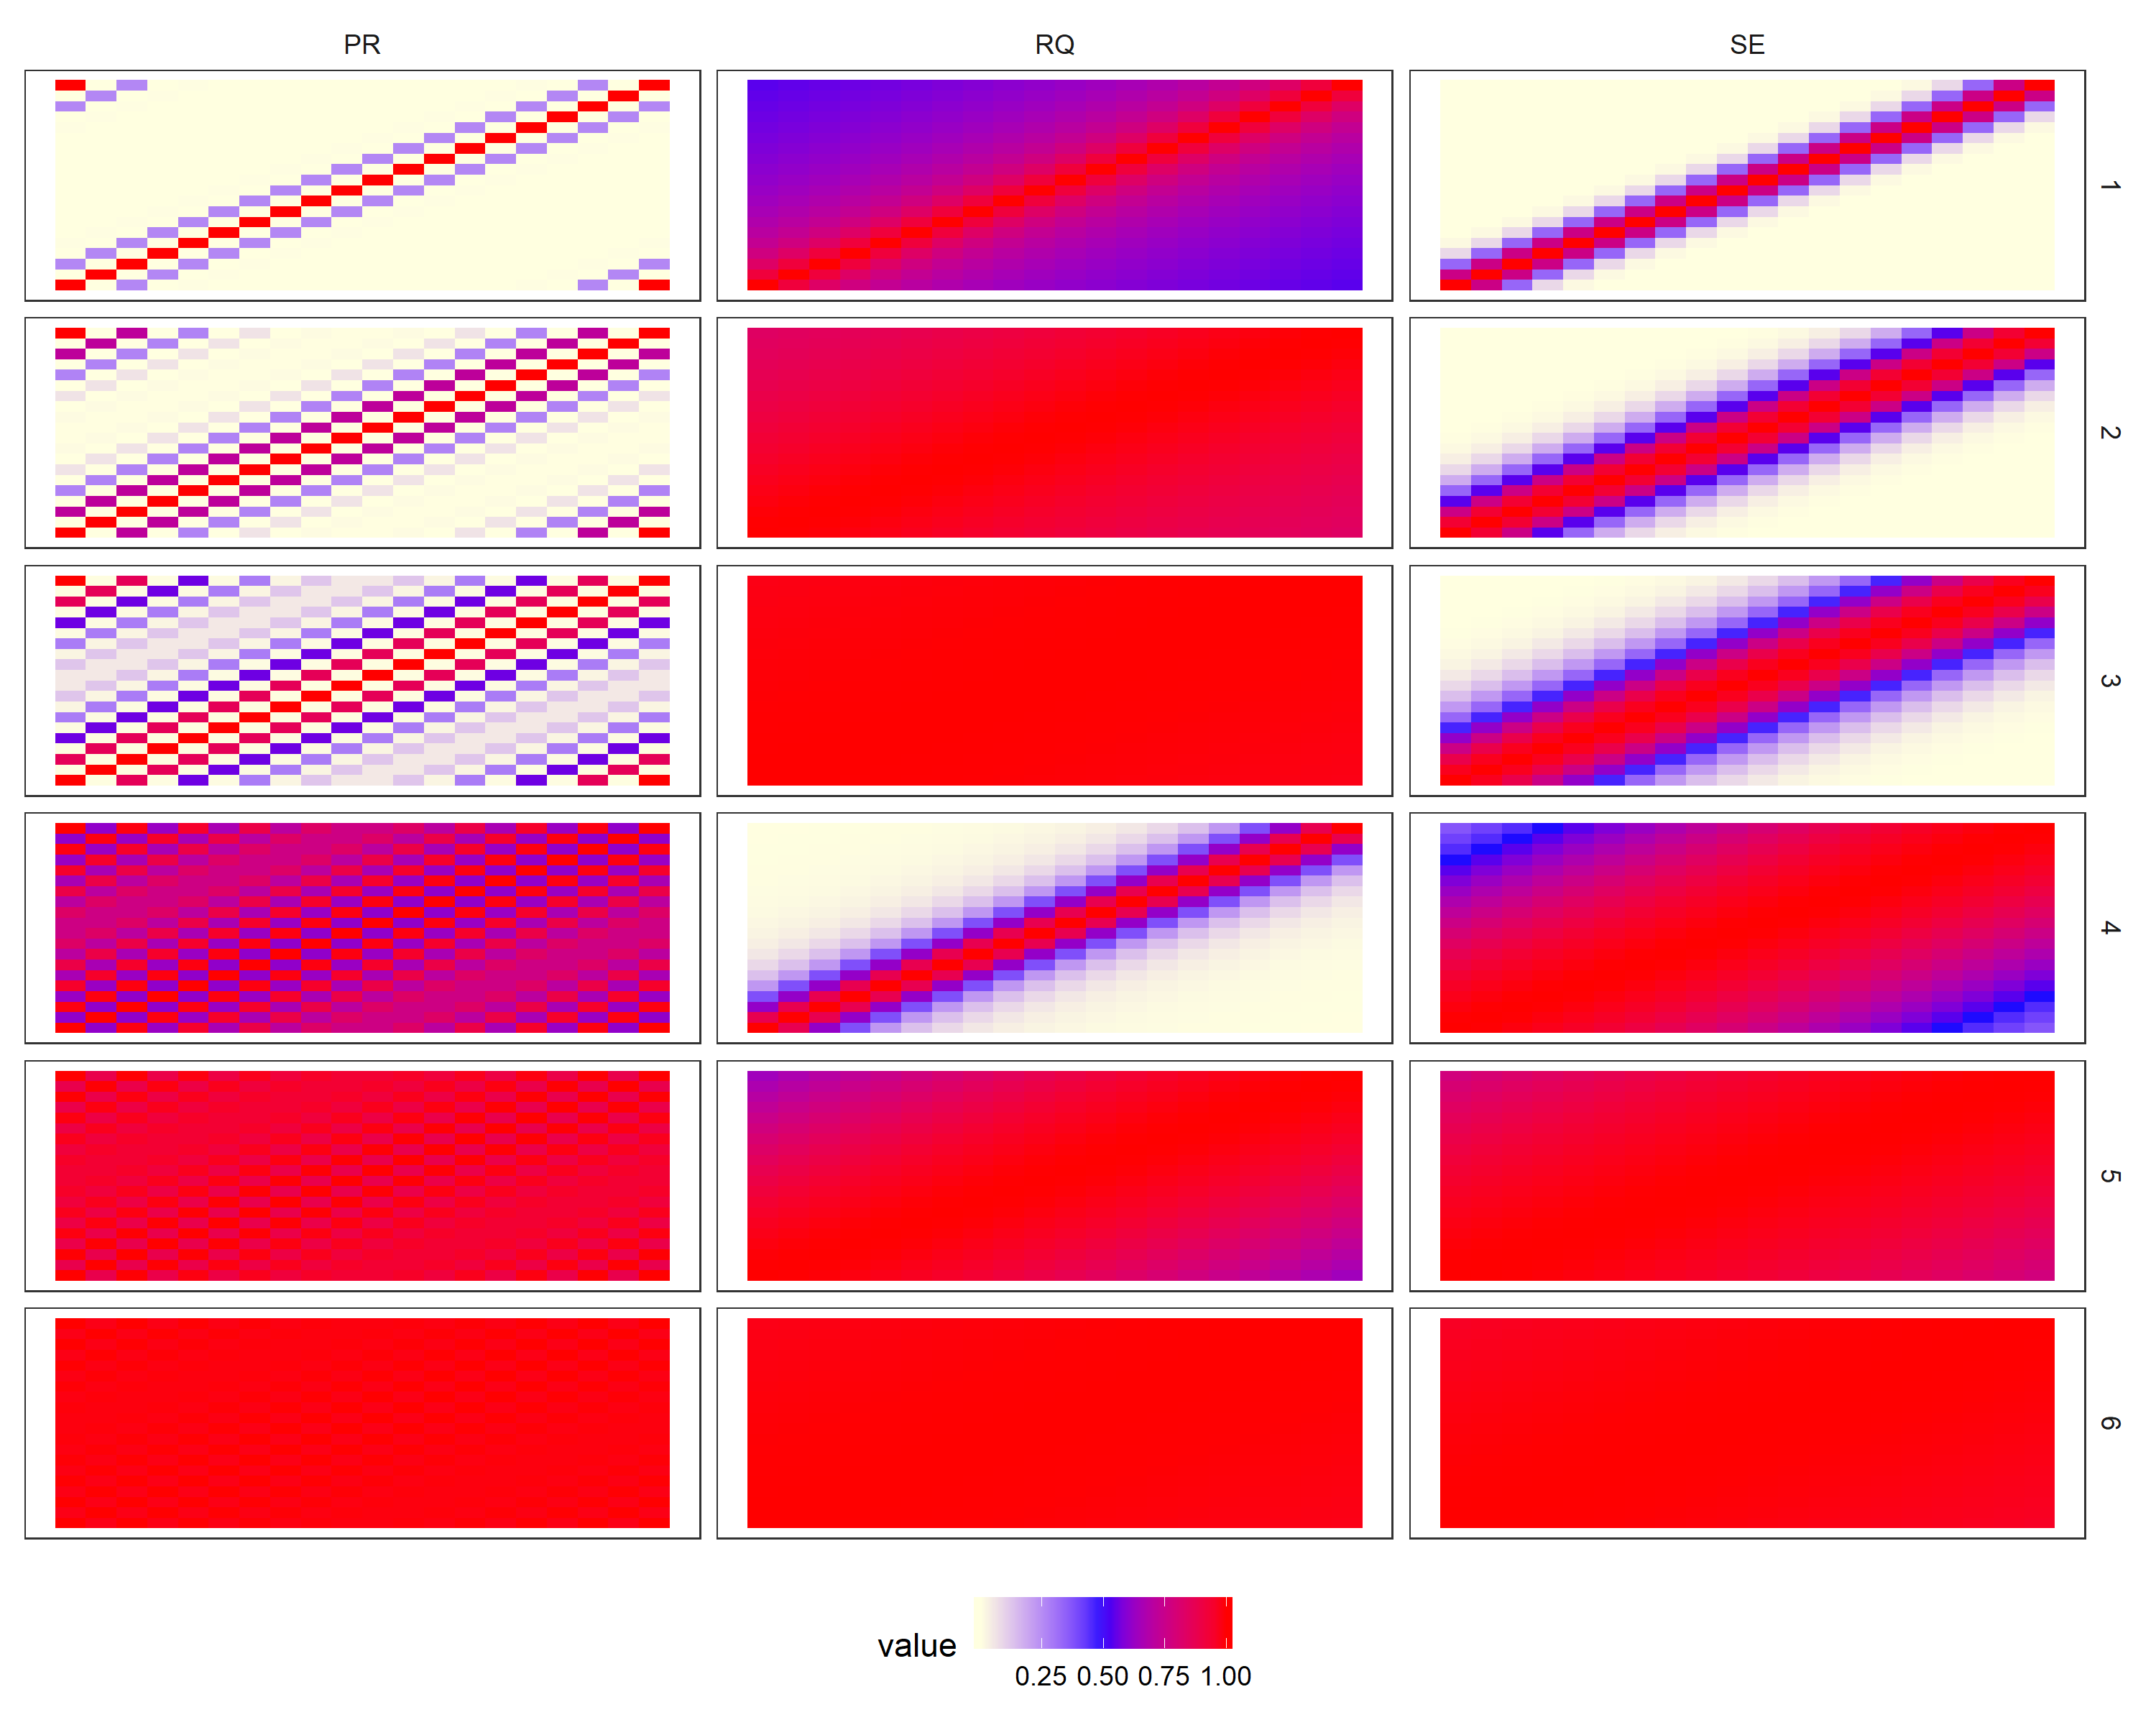
\includegraphics[scale = 0.15]{GP_illustrations/kernel_stationary.png}
\caption{Stationary kernels under 6 different sets of hyper-parameters.}\label{fig:}
\end{figure}

\begin{figure}[H]
\centering
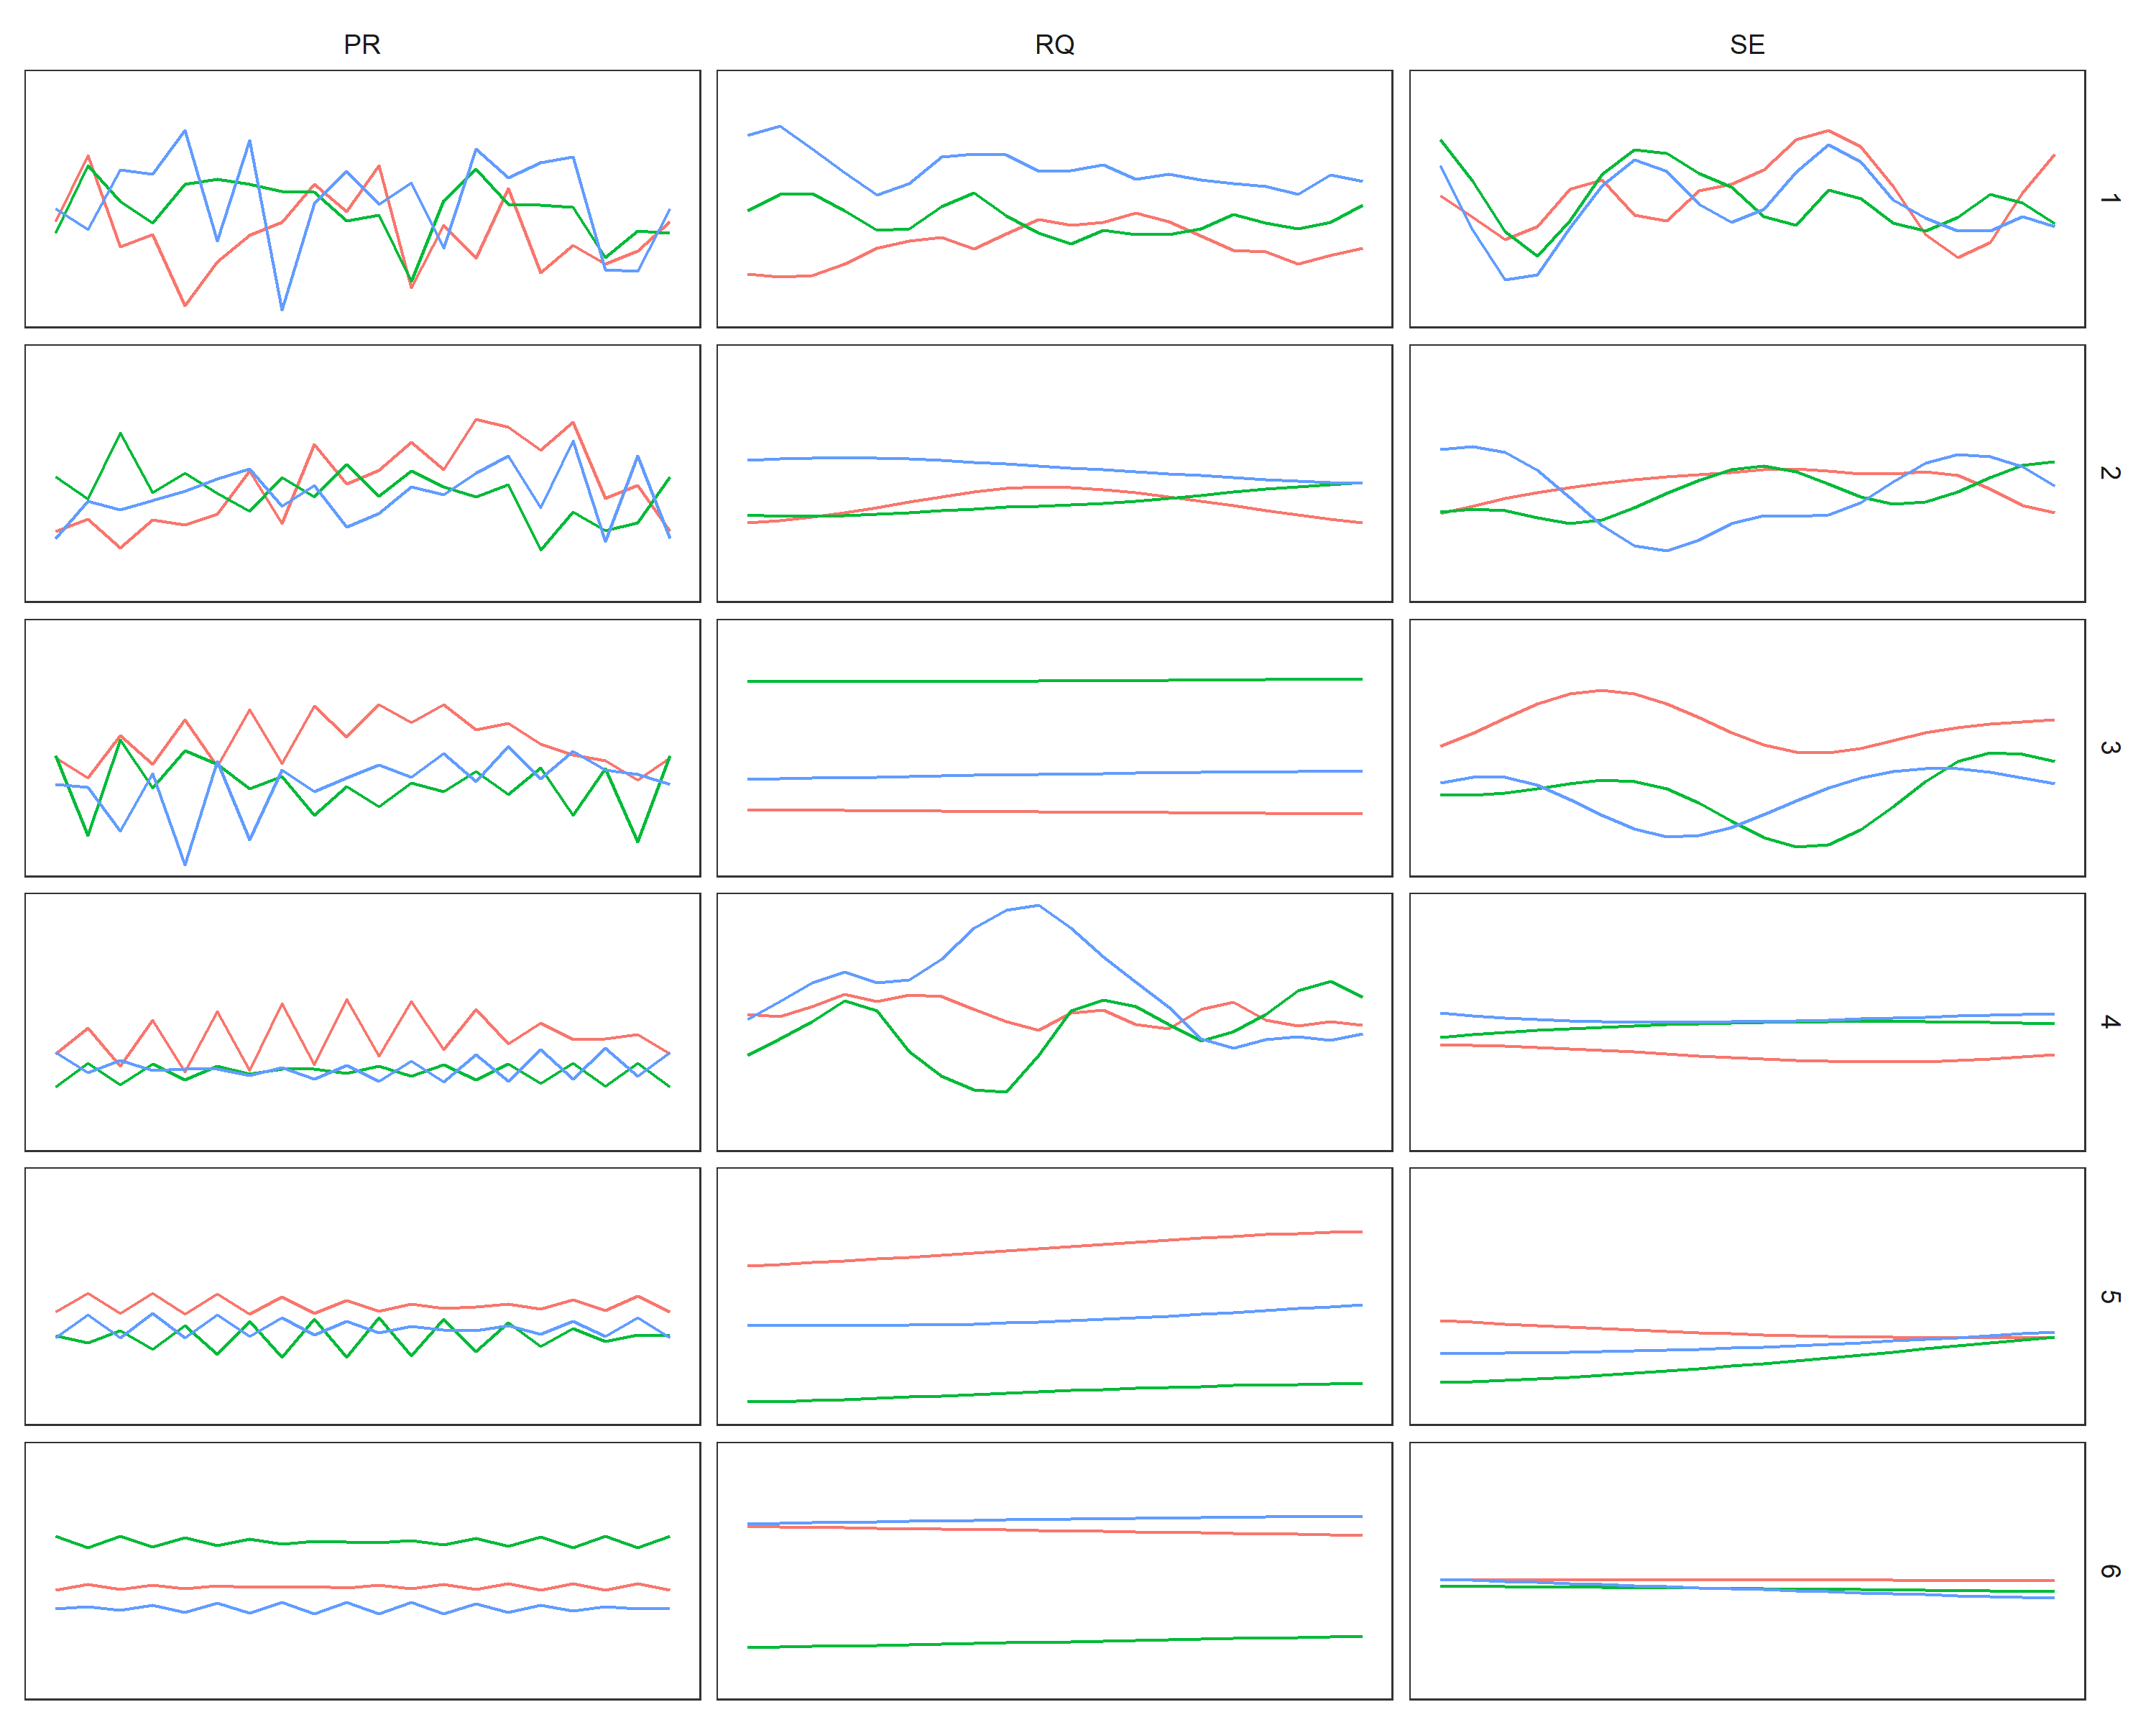
\includegraphics[scale = 0.15]{GP_illustrations/y_sim_stationary.png}
\caption{The 3 path of the signal $c_k$ simulated from the a priori distribution in Equation \eqref{eq:model_IMF_GP_k} under different stationary kernel assumptions (columns wise) and for 6 different sets of hyper-parameters.}\label{fig:}
\end{figure}

\begin{figure}[H]
\centering
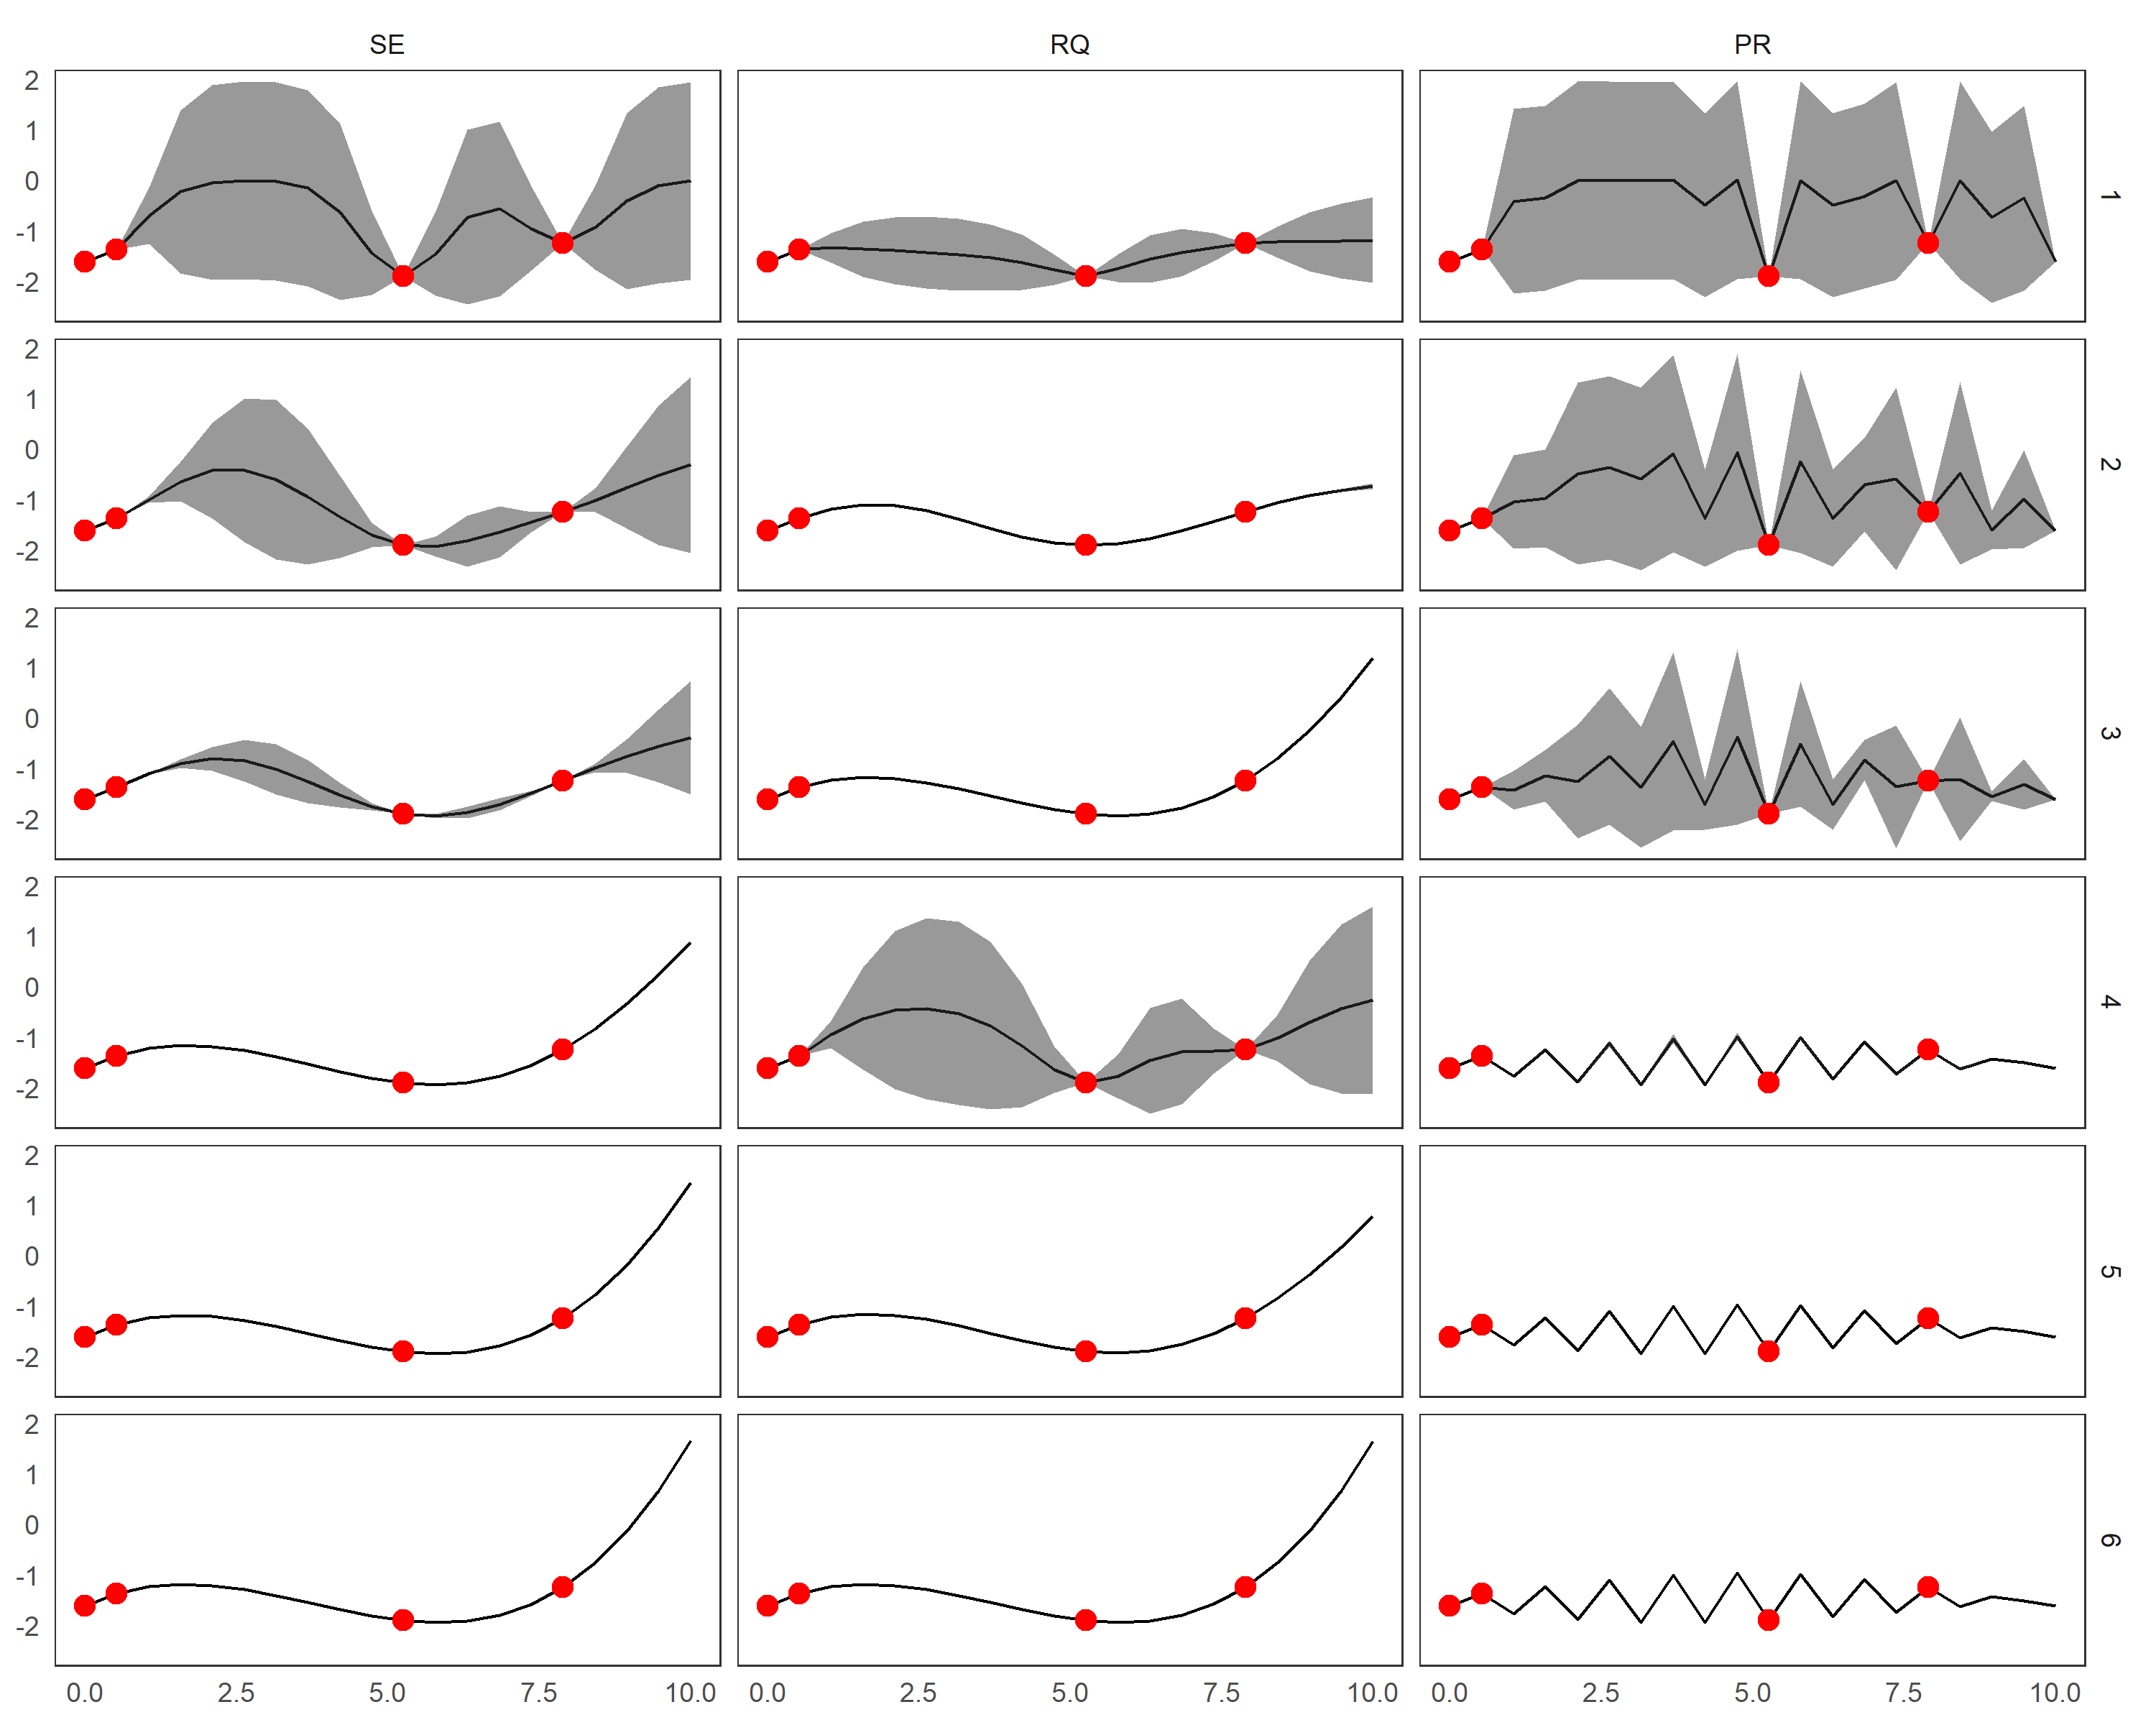
\includegraphics[scale = 0.15]{GP_illustrations/y_pred_stationary.png}
\caption{The predictive conditional mean of the IMF with the confidence intervals  under  noise-free assumption for different stationary kernel assumptions (columns wise) given 6 different sets of hyper-parameters. The red dots correspond to the observed values of the signal}\label{fig:}
\end{figure}
\subsection{Estimation of the Static Parameters}
\subsubsection{MLE Estimation of the Static Parameters in Gaussian Processes Models}
In the following subsection we derive the MLE estimator of the vectors of parameters $\varphi_k$ and $\Psi_k$.  Given the model in Equation \eqref{eq:model_IMF_GP_k_noisy}, the loglikelihood of the the observation set $\big\{\mathbf{c}_k, \mathbf{t}\big\}$ is the following 
\begin{equation}\label{eq:IMF_loglik_noisy}
l_k\Big( \mathbf{c}_k, \mathbf{t} , \varphi_k, \Psi_k \Big) = - \frac{N}{2} \log 2 \pi - \frac{1}{2} \log |\mathbf{K}_k + \sigma^2_k \mathbb{I}_N | - \frac{1}{2}\mathbf{v}_k^T \Big(\mathbf{K}_k   + \sigma^2_k \mathbb{I}_N \Big)^{-1} \mathbf{v}_k
\end{equation}
where $\mathbf{v}_k = \mathbf{c}_k - \bm{\mu}_k$ and $\mathbf{K}_k$ denotes a $N \times N$ Gram matrix defined as
\begin{align*}
\mathbf{K}_{k}  := K_{k} (\mathbf{t},\mathbf{t}) = \begin{bmatrix}
K_k (\mathbf{t}^{(1)},\mathbf{t}^{(1)}  )& K_k (\mathbf{t}^{(1)},\mathbf{t}^{(2)}  ) & \cdots & K_k (\mathbf{t}^{(1)},\mathbf{t}^{(M-1)}  ) & K_k (\mathbf{t}^{(1)},\mathbf{t}^{(M)}  ) \\
K_k (\mathbf{t}^{(2)},\mathbf{t}^{(1)}  )& K_k (\mathbf{t}^{(2)},\mathbf{t}^{(2)}  ) & \cdots & K_k (\mathbf{t}^{(2)},\mathbf{t}^{(M-1)}  ) & K_k (\mathbf{t}^{(2)},\mathbf{t}^{(M)}  ) \\
\vdots & \vdots & \ddots & \vdots & \vdots  \\
K_k (\mathbf{t}^{(M-1)},\mathbf{t}^{(1)}  )& K_k (\mathbf{t}^{(M-1)},\mathbf{t}^{(2)}  ) & \cdots & K_k (\mathbf{t}^{(M-1)},\mathbf{t}^{(M-1)}  ) & K_k (\mathbf{t}^{(M-1)},\mathbf{t}^{(M)}  ) \\
K_k (\mathbf{t}^{(M)},\mathbf{t}^{(1)}  )& K_k (\mathbf{t}^{(M)},\mathbf{t}^{(2)}  ) & \cdots & K_k (\mathbf{t}^{(M)},\mathbf{t}^{(M-1)}  ) & K_k (\mathbf{t}^{(M)},\mathbf{t}^{(M)}  ) 
\end{bmatrix}_{N \times N}, 
\end{align*}
If the sets of points $\mathbf{t}^{(i)}$ are the same and equal to $\mathbf{t}^*$, the vector $\mathbf{t}$ is constructed by stacking $\mathbf{t}^*$ by $M$ times. Then the formulation of the likelihood simplifies to 
\begin{equation}
l_k\Big( \mathbf{c}_k, \mathbf{t}^* , \varphi_k, \Psi_k \Big) = - \frac{N}{2} \log 2 \pi - \frac{M}{2} \log |K_k (\mathbf{t}^*,\mathbf{t}^*  ) + \sigma^2_k \mathbb{I}_{N_*} | - \frac{1}{2}\sum_{i = 1}^M \mathbf{v}^{(i) \ T} \Big( K_k (\mathbf{t}^*,\mathbf{t}^*  ) +  + \sigma^2_k \mathbb{I}_{N_*} \Big)^{-1}\mathbf{v}^{(i)} \big) 
\end{equation}
Under the formulation of the loglikelihood in Equation \eqref{eq:IMF_loglik_noisy}, the static parameters of the model in Equation \eqref{eq:model_IMF_GP_k_noisy} can be estimated by solving the system of equations given by
\begin{equation}
\nabla l_k\Big( \mathbf{c}_k, \mathbf{t} , \varphi_k, \Psi_k \Big)  = \mathbf{0}
\end{equation}
where $\nabla l_k\Big( \mathbf{c}_k, \mathbf{t} , \varphi_k, \Psi_k \Big) $ denotes the gradient of the loglikelihood with respect to the vector of static parameters given by
\begin{align*}
& \frac{\partial l_k\Big( \mathbf{c}_k, \mathbf{t} , \varphi_k, \Psi_k \Big)}{\partial \varphi_k} = \frac{1}{2} = \mathbf{c}_k \Big(\mathbf{K}_k + \sigma^2_k \mathbb{I}_N\Big)^{-1} \mathbf{v}_k \frac{\partial \mu_k(\mathbf{t})}{\partial \varphi_k} \\
& \frac{\partial l_k\Big( \mathbf{c}_k, \mathbf{t} , \varphi_k, \Psi_k \Big)}{\partial \Psi_k} = \frac{1}{2} \tr \bigg\{\bigg(\Big(\mathbf{K}_k + \sigma^2_k \mathbb{I}_N\Big)^{-1}  \mathbf{v}_k \mathbf{v}_k^T\Big(\mathbf{K}_k + \sigma^2_k \mathbb{I}_N\Big)^{-1} -\Big(\mathbf{K}_k + \sigma^2_k \mathbb{I}_N\Big)^{-1}  \bigg) \frac{\partial \mathbf{K}_k }{ \partial \Psi_k} \bigg\} \\
& \frac{\partial l_k\Big( \mathbf{c}_k , \mathbf{t} , \varphi_k, \Psi_k \Big)}{\partial \sigma^2_k} = \frac{1}{2} \tr \bigg\{\bigg(\mathbf{K}_k + \sigma^2_k \mathbb{I}_N\Big)^{-1}  \mathbf{v}_k \mathbf{v}_k^T\Big(\mathbf{K}_k + \sigma^2_k \mathbb{I}_N\Big)^{-1} -\Big(\mathbf{K}_k + \sigma^2_k \mathbb{I}_N\Big)^{-1}  \bigg\} \\
\end{align*}

\subsubsection{Kernel Alignment}


\subsubsection{Estimators of the Static Parameters given Splines Formulation of $x(t)$}
\input{IMF_pred_distribution}
\subsection{Multikernel Representation of the Signal}

\subsubsection{Assuming Independence of IMFS }
Given the Gaussian Process model of the $c_k(t)$, the distribution of $x(t)$ can be formulated as a uniform mixture of Gaussian Processes with different kernels.  Again, we can either assume that the observed values are or are not perturbed by a noise. In the following derivation we assume that the model of the $x(t)$ includes additional  term corresponding to the zero mean Gaussian noise with variance $\sigma^2$, that is
\begin{equation}
x(t) = \sum_{k = 1}^K c_k(t) + r_K(t) + \epsilon
\end{equation}
and results in the following distribution of $x(t)$ 
\begin{equation}
x(t) \sim ~   GP \bigg(r_K(t) + \sum_{k=1}^K \mu_k(t); \sum_{k=1}^K K_k(t,t') + \sigma^2 \bigg) 
\end{equation}
The scalar $\sigma^2$ can be estimated by MLE of $x(t)$, given its $M$ realization, $\mathbf{x}^{(i)}$, formed into a vector $\mathbf{x} = \big[\mathbf{x}^{(1)},\ldots, \mathbf{x}^{(M)} \big]$. If we denote by $K(t,t') := \sum_{k=1}^K K_k(t,t')$ a vector operator similarly defined as $K_k(t,t')$  and by $\mu(t) = r_K(t) + \sum_{k=1}^K \mu_k(t)$, then the log-likelihood of the model 
\begin{equation}
l\big( \mathbf{x}, \mathbf{t} , \sigma^2 \big) = - \frac{N}{2} \log 2 \pi - \frac{1}{2} \log |K(\mathbf{t},\mathbf{t}) + \sigma^2 \mathbb{I}_N | - \frac{1}{2}(\mathbf{x} - \mu(\mathbf{t}))^T \Big(K(\mathbf{t},\mathbf{t})   + \sigma^2 \mathbb{I}_N \Big)^{-1} (\mathbf{x} - \mu(\mathbf{t}))
\end{equation}
with corresponding gradient
\begin{equation*}
\frac{\partial l\big( \mathbf{x} , \mathbf{t} , \sigma^2 \big)}{\partial \sigma^2} = \frac{1}{2} \tr \bigg\{\Big(K(\mathbf{t},\mathbf{t}) + \sigma^2 \mathbb{I}_N\Big)^{-1}  (\mathbf{x} - \mu(\mathbf{t}))(\mathbf{x} - \mu(\mathbf{t}))^T\Big(K(\mathbf{t},\mathbf{t})  + \sigma^2 \mathbb{I}_N\Big)^{-1} -\Big(K(\mathbf{t},\mathbf{t})+ \sigma^2 \mathbb{I}_N\Big)^{-1}  \bigg\} 
\end{equation*}
The predictive distribution of $x(t)$ is given by 
\begin{equation*}
\mathbb{E}_{x(t)| \mathbf{t}} \big[x(\mathbf{s})] = \sum_{k = 1}^K \mathbb{E}_{c_k(t)|\mathbf{t}} \big[c_k(\mathbf{s})] 
\end{equation*}
and the covariance matrix given by
\begin{equation*}
\mathbf{Cov}_{x(t)|\mathbf{t}} \big[x(\mathbf{s})]  = \sum_{k = 1}^K\mathbf{Cov}_{c_k(t)|\mathbf{t}} \big[c_k(\mathbf{s})]  + \sigma^2
\end{equation*}


\subsubsection{Correlation of IMFS }
If the GP of $c_k$ are not independent, the Gram matrix of the model for $x(t)$ would contain additional elements which provide the correlation structure between different IMFs
\begin{equation}
x(t) \sim ~   GP \bigg(r_K(t) + \sum_{k=1}^K m_k(t); \sum_{k=1}^K K_k(t,t') + 2\sum_{k_1,k_2=1, k_1<k_2}^K K_{k1,k2}(t,t') + \sigma^2 \bigg) 
\end{equation}
where $K_{k1,k2}(t,t')$ defines the dependence structure between $c_{k_1}(t)$ and $c_{k_2}(t)$

\section{Brownian Bridge Analogue to  construct IMFs}
GP representation does not ensures itself that the predicted function from a given Gaussian process is IMF , that is, it satisfies (I1)-(I2). Therefore, we explire the following approches

Weiner process is a zero mean non-stationary Gaussian Process with the kernel $K(t,t') = min(t,t')$, that is
\begin{equation}
W(t) \sim \text{GP}(0,K(t,t'))
\end{equation}
The Brownian Bridge for $t \in [0,T]$ is defined as
\begin{equation}
B(t) = W(t) - \frac{t}{T} W(T)
\end{equation}
Therefore, it is also the Gaussian Process which is zero mean and has the covariance kernel equals to
\begin{align*}
\mathbf{Cov}(B(t),B(s)) & = \mathbf{Cov}(W(t),W(s)) - \frac{s}{T} \mathbf{Cov}(W(t),W(T)) - \frac{t}{T} \mathbf{Cov}(W(s),W(T)) + \frac{st}{T^2} \mathbf{Cov}(W(T),W(T))\\
& = K(t,s) - \frac{s}{T} K(t,T) - \frac{t}{T} K(T,s) + \frac{ts}{T^2} K(T,T)\\
&  = min(t,t') - \frac{ts}{T}
\end{align*}
The described process $B(t)$ satisfies that $B(0) = B(T) = 0$. The Brownian bridge which statisfied 
$B(t_0) = a$ and $B(_t1) = b$ is a solution to the following SDE system of equations
\begin{equation}
\begin{cases}
& dB(t) = dW(t) \\
& B(t_0) = a \\
& B(t_1) = b
\end{cases},  \text{ for } t_0 \leq t \leq t_1
\end{equation}
Therefore, the Brownian Bridge

and after calculations results in the form
\begin{equation}
B(t) = a + (b-a)\frac{t}{T} + W(t) - \frac{t}{T} W(T)
\end{equation} 
and therefore it is a Gaussian Process 
\begin{equation}
B(t) \sim \text{GP}\Big( a + (b-a)\frac{t}{T} ,K(t,t') - \frac{tt'}{T} \Big)
\end{equation}
for $0 \leq t \leq T$
%%%  https://math.aalto.fi/reports/a481.pdf
%% https://www.diva-portal.org/smash/get/diva2:233650/FULLTEXT01.pdf
\subsubsection{Brownian Bridge Movement Model}

Let $W(t)$ denote the Brownian Motion such that
\begin{equation}
W(t) \sim \mathcal{GP}, \big(0,k(t,t') \big)
\end{equation}
with the kernel function $k(t,t') =  \min \big\{ t,t'\big\} $ and $t \in [0,T]$. Let us define the sequence of $N$ points $0 \leq t_1 < t_2 < \ldots <t_N \leq < T$ such that we require that the process $W(t)$ had the fixed values at that points $W(t_i) = a_i$ for $ i \in \big\{1,\ldots,N \big\}$.  Theretofore, we are looking for a Gaussian process for $t \in [0,T]$ model of a conditional variable defined as 
\begin{equation}
B(t) := W(t) | W(t_1) = a_1, W(t_2) = a_2, \ldots, ... W(t_N) = a_N
\end{equation} 
Let $\mathbf{W} = \big[W(t_1) , W(t_2) , \ldots, ... W(t_N)  \big]$ and $\mathbf{t} = \big[ t_1, t_2, \ldots, t_N \big]$ be $N$-dimensional vectors.  Since $W(t)$ is a Gaussian Process, the random variable $W(t) | W(t_1) , W(t_2) , \ldots, ... W(t_N) $ is also a Gaussian Process with the conditional mean
\begin{equation}
\mu(t) : = \mathbb{E}_{W(t) | W(t_1) , W(t_2) , \ldots, ... W(t_N) }\big[ W(t) \big] = \mathbf{k} \big( t, \mathbf{t} \big)^T \mathbf{K}(\mathbf{t},\mathbf{t} \big)^{-1} \mathbf{W}
\end{equation}
and the covariance function 
\begin{equation}
\k(t,t') = \mathbb{E}_{W(t) | W(t_1) , W(t_2) , \ldots, ... W(t_N) }\Big[ \big[ W(t) -\mu(t)  \big] \big[W(t')  -\mu(t')  \big] \big] \Big] =k(t,t') -  \mathbf{k} \big( t, \mathbf{t} \big)^T \mathbf{K}(\mathbf{t},\mathbf{t} \big)^{-1}   \mathbf{k} \big( t', \mathbf{t} \big)
\end{equation}

where
\begin{equation}
\mathbf{K}(\mathbf{t},\mathbf{t}): =\begin{bmatrix}
t_1 & t_1 & t_1 & \ldots & t_1 \\
t_1 & t_2 & t_2 & \ldots & t_2 \\
t_1 & t_2 & t_3 & \ldots & t_3 \\
\vdots & \vdots & \ddots & \vdots \\
t_1 & t_2 & t_3 & \vdots & t_N
\end{bmatrix}_{N \times N}
\end{equation}
and 
\begin{equation}
\mathbf{k}(t,\mathbf{t}): =\begin{bmatrix}
\min(t,t_1) \\
\min(t,t_2) \\
\vdots \\
\min(t,t_N)
\end{bmatrix}_{N \times 1}
\end{equation}


\subsection{Symmetric Local Extremas of IMFs} 
On every time internal there is a Brownian bridge or constrained Brownian bridge which starts and end from local extrema which are $x^{min} (t)= -x^{max}(t)$ for $t \in [\tau_i,\tau_{i+1}$
\subsection{Nonsymmetric}

\subsection{Bayesian EMD}
1. Construct a set of functions in Bayesian setting to have a IMF representation with restricted posterior (what needs to be satisfied on maxima and minima and how to ensure it)
2. Analogous of Brownian Bridge IMFs in Bayesian setting

Berger's optimal theory. Books on smoothing


%%\appendix
\label{appendix_IMFS-coeff}
Proofs of the IMFs coefficients\\
Consider D iteration of the sifting process (i.e. producing D IMFs). The $D-th$ IMF can be represented by a spline whose coefficients are a linear combination of the coefficients of $S(t)$ and the coefficients of the mean envelopes  of the previous extracted IMFs. By taking into account the first sifting process, we show the above statement and then extend it to the $D-th$ case.\\

Consider the spline interpolating the original set of data $x(t)$, i.e. $S(t)$. 
By being at the initial step of the sifting procedure, i.e. step $0$, we modify such equation:

\begin{equation}
S(t) = \sum_{i=1}^{n-1} \left(a_i^0 t^3 +b_i^0 t^2 + c_i^0 t +d_i^0 \right) \mathbbm{1} \left( t \in \left[ t_{i-1},t_i \right] \right) 
\end{equation} 

where the upper indices of the coefficients state the step at which the sifting procedure is. Consider the upper and lower envelope of $S(t)$ defined in \ref{upper_env} and \ref{lower_env}. Such splines are evaluated at times of the original spline $S(t)$, i.e. at $t$, as:

\begin{equation}
S\left( e_1^S \right) = \sum_{j=1}^{N-1} \left( a_{j,0}^{e_1} t^3 + b_{j,0}^{e_1} t^2 + c_{j,0}^{e_1} t +d_{j,0}^{e_1} \right) \mathbbm{1} \left(t \in \left[t_{j-1}, t_j \right] \right)
\end{equation}

\begin{equation}
S\left( e_2^S \right) = \sum_{j=0}^{n-1} \left( a_{j,0}^{e_2} t^3 + b_{j,0}^{e_2} t^2 + c_{j,0}^{e_2} t +d_{j,0}^{e_2} \right) \mathbbm{1} \left(t \in \left[t_{j-1}, t_j \right] \right)
\end{equation}

Let us put $S(t) = c_0$ and $m_{1,0} = \frac{S(e_1^S) + S(e_2^S)}{2}$ its mean envelope, where the first index corresponds to the number of the IMF that the sifting procedure is extracting (the first one here) and the second one the step of this sifting. Consider a simple example where $n=3$ and the number of steps of the sifting equal to 2.\\
The above definitions can be represented by:
\begin{equation}
\begin{split}
c_0 = S(t) = \sum_{i=1}^{N-1} \left(a_i^0 t^3 +b_i^0 t^2 + c_i^0 t +d_i^0 \right) \mathbbm{1} \left( t \in \left[ t_{i-1},t_i \right] \right) = \\
a_1^0 t_1^3 + b_1^0 t_1^2 + c_1^0 t_1 + d_1^0 + a_2^0 t_2^3 + b_2^0 t_2^2 + c_2^0 t_2 + d_2^0 
\end{split} 
\end{equation}

\begin{equation}
\begin{split}
m_{1,0} =  \frac{S(e_1^S) + S(e_2^S)}{2} = \frac{1}{2} \left[ a_{1,0}^{e_1} t_1^3 + b_{1,0}^{e_1} t_1^2 + c_{1,0}^{e_1} t_1 + d_{1,0}^{e_1} + a_{2,0}^{e_1} t_2^3 + b_{2,0}^{e_1} t_2^2 + c_{2,0}^{e_1} t_2 + d_{2,0}^{e_1} \right] + \\
\left[ a_{1,0}^{e_2} t_1^3 + b_{1,0}^{e_2} t_1^2 + c_{1,0}^{e_2} t_1 + d_{1,0}^{e_2} + a_{2,0}^{e_2} t_2^3 + b_{2,0}^{e_2} t_2^2 + c_{2,0}^{e_2} t_2 + d_{2,0}^{e_2} \right]
\end{split}
\end{equation}

We look at the first step of the first sifting procedure computed by $c_0 - m_{1,0}$. By rearranging and grouping we obtain:
\begin{equation}
\label{first_ext}
\begin{split}
c_0 - m_{1,0} = \left[ a_{1,0} - \frac{1}{2} \left( a_{1,0}^{e_1} + a_{1,0}^{e_2}  \right) \right] t_1^3 + \left[ a_{2,0} - \frac{1}{2} \left( a_{2,0}^{e_1} + a_{2,0}^{e_2}  \right) \right] t_2^3 + \\
\left[ b_{1,0} - \frac{1}{2} \left( b_{1,0}^{e_1} + b_{1,0}^{e_2}  \right) \right] t_1^2 + \left[ b_{2,0} - \frac{1}{2} \left( b_{2,0}^{e_1} + b_{2,0}^{e_2}  \right) \right] t_2^2 + \\
\left[ c_{1,0} - \frac{1}{2} \left( c_{1,0}^{e_1} + c_{1,0}^{e_2}  \right) \right] t_1 + \left[ c_{2,0} - \frac{1}{2} \left( c_{2,0}^{e_1} + c_{2,0}^{e_2}  \right) \right] t_2 + \\
\left[ d_{1,0} - \frac{1}{2} \left( d_{1,0}^{e_1} + d_{1,0}^{e_2}  \right) \right] + \left[ d_{2,0} - \frac{1}{2} \left( d_{2,0}^{e_1} + d_{2,0}^{e_2}  \right) \right]
\end{split}
\end{equation}

To then consider the second (and last in this simple case) step of the sifting extracting the first IMF, consider the following equalities:

\begin{multicols}{2}
\begin{itemize}
\item $a_1^1 = a_{1,0} - \frac{1}{2} \left( a_{1,0}^{e_1} + a_{1,0}^{e_2}  \right)$
\item $a_2^1 = a_{2,0} - \frac{1}{2} \left( a_{2,0}^{e_1} + a_{2,0}^{e_2} \right) $
\item $b_1^1 = b_{1,0} - \frac{1}{2} \left( b_{1,0}^{e_1} + b_{1,0}^{e_2}  \right)$
\item $b_2^1 = b_{2,0} - \frac{1}{2} \left( b_{2,0}^{e_1} + b_{2,0}^{e_2}  \right) $
\item $ c_1^1 = c_{1,0} - \frac{1}{2} \left( c_{1,0}^{e_1} + c_{1,0}^{e_2}  \right)$
\item $c_2^1 =  c_{2,0} - \frac{1}{2} \left( c_{2,0}^{e_1} + c_{2,0}^{e_2}  \right)  $
\item $d_1^1 = d_{1,0} - \frac{1}{2} \left( d_{1,0}^{e_1} + d_{1,0}^{e_2}  \right)$
\item $d_2^1 = d_{2,0} - \frac{1}{2} \left( d_{2,0}^{e_1} + d_{2,0}^{e_2}  \right)$
\end{itemize}
\end{multicols}

By substituting the above equalities in \ref{first_ext}, the next result is obtained:
\begin{equation}
c_0 - m_{0,0} = a_1^1 t_1^3 + a_2^1 t_2^3 + b_1^1 t_1^2 + b_2^1 t_2^2 + c_1^1 t_1 + c_2^1 t_2 + d_1^1 + d_2^1 
\end{equation}

Define this intermediate step as $h_{1,1} = c_0 - m_{1,0}$ where the extracted component $h_{1,1}$ is not a final IMF yet. Therefore, the algorithm keeps running. At this stage, the mean envelope is given by $m_{1,1} = \frac{S(e_1^{h_{1,1}})+S(e_2^{h_{1,1}})}{2}$. The second step of the sifting is:
\begin{equation}
\label{second_extr}
\begin{split}
h_{1,2} = h_{1,1} - m_{1,1} = \left[ a_{1,1} - \frac{1}{2} \left( a_{1,1}^{e_1} + a_{1,1}^{e_2}  \right) \right] t_1^3 + \left[ a_{2,1} - \frac{1}{2} \left( a_{2,1}^{e_1} + a_{2,1}^{e_2}  \right) \right] t_2^3 + \\
\left[ b_{1,1} - \frac{1}{2} \left( b_{1,1}^{e_1} + b_{1,1}^{e_2}  \right) \right] t_1^2 + \left[ b_{2,1} - \frac{1}{2} \left( b_{2,1}^{e_1} + b_{2,1}^{e_2}  \right) \right] t_2^2 + \\
\left[ c_{1,1} - \frac{1}{2} \left( c_{1,1}^{e_1} + c_{1,1}^{e_2}  \right) \right] t_1 + \left[ c_{2,1} - \frac{1}{2} \left( c_{2,1}^{e_1} + c_{2,1}^{e_2}  \right) \right] t_2 + \\
\left[ d_{1,1} - \frac{1}{2} \left( d_{1,1}^{e_1} + d_{1,1}^{e_2}  \right) \right] + \left[ d_{2,1} - \frac{1}{2} \left( d_{2,1}^{e_1} + d_{2,1}^{e_2}  \right) \right]
\end{split}
\end{equation}

Define the following equalities:

\begin{multicols}{2}
\begin{itemize}
\item $a_1^2 = a_{1,1} - \frac{1}{2} \left( a_{1,1}^{e_1} + a_{1,1}^{e_2}  \right)$
\item $a_2^2 = a_{2,1} - \frac{1}{2} \left( a_{2,1}^{e_1} + a_{2,1}^{e_2} \right) $
\item $b_1^2 = b_{1,1} - \frac{1}{2} \left( b_{1,1}^{e_1} + b_{1,1}^{e_2}  \right)$
\item $b_2^2 = b_{2,1} - \frac{1}{2} \left( b_{2,1}^{e_1} + b_{2,1}^{e_2}  \right) $
\item $ c_1^2 = c_{1,1} - \frac{1}{2} \left( c_{1,1}^{e_1} + c_{1,1}^{e_2}  \right)$
\item $c_2^2 =  c_{2,1} - \frac{1}{2} \left( c_{2,1}^{e_1} + c_{2,1}^{e_2}  \right)  $
\item $d_1^2 = d_{1,1} - \frac{1}{2} \left( d_{1,1}^{e_1} + d_{1,1}^{e_2}  \right)$
\item $d_2^2 = d_{2,1} - \frac{1}{2} \left( d_{2,1}^{e_1} + d_{2,1}^{e_2}  \right)$
\end{itemize}
\end{multicols}

Substituting them within \ref{second_extr} provides the next equation:
\begin{equation}
h_{1,2} = h_{1,1} - m_{1,1} = a_1^2 t_1^3 + a_2^2 t_2^3 + b_1^2 t_1^2 + b_2^2 t_2^2 + c_1^2 t_1 + c_2^2 t_2 + d_1^2 + d_2^2 
\end{equation}

This corresponds to the first extracted IMF, i.e. $c_1 = h_{1,2}$. By considering the above equation and substituting all the equalities that we have taken into account, we get:
\begin{equation}
\label{c_1}
\begin{split}
c_1 = \left[ a_{1,0} - \frac{1}{2} \left(a_{1,0}^{e_1} + a_{1,0}^{e_2} \right) - \frac{1}{2} \left(a_{1,1}^{e_1} + a_{1,1}^{e_2} \right)  \right] t_1^3 + \left[ a_{2,0} - \frac{1}{2} \left(a_{2,0}^{e_1} + a_{2,0}^{e_2} \right) - \frac{1}{2} \left(a_{2,1}^{e_1} + a_{2,1}^{e_2} \right)  \right] t_2^3 \\
+ \left[ b_{1,0} - \frac{1}{2} \left(b_{1,0}^{e_1} + b_{1,0}^{e_2} \right) - \frac{1}{2} \left(b_{1,1}^{e_1} + b_{1,1}^{e_2} \right)  \right] t_1^2 + \left[ b_{2,0} - \frac{1}{2} \left(b_{2,0}^{e_1} + b_{2,0}^{e_2} \right) - \frac{1}{2} \left(b_{2,1}^{e_1} + b_{2,1}^{e_2} \right)  \right] t_2^2 \\
+ \left[ c_{1,0} - \frac{1}{2} \left(c_{1,0}^{e_1} + c_{1,0}^{e_2} \right) - \frac{1}{2} \left(c_{1,1}^{e_1} + c_{1,1}^{e_2} \right)  \right] t_1 + \left[ c_{2,0} - \frac{1}{2} \left(c_{2,0}^{e_1} + c_{2,0}^{e_2} \right) - \frac{1}{2} \left(c_{2,1}^{e_1} + c_{2,1}^{e_2} \right)  \right] t_2 \\
+ \left[ d_{1,0} - \frac{1}{2} \left(d_{1,0}^{e_1} + d_{1,0}^{e_2} \right) - \frac{1}{2} \left(d_{1,1}^{e_1} + d_{1,1}^{e_2} \right)  \right] + \left[ d_{2,0} - \frac{1}{2} \left(d_{2,0}^{e_1} + d_{2,0}^{e_2} \right) - \frac{1}{2} \left(d_{2,1}^{e_1} + d_{2,1}^{e_2} \right)  \right] 
\end{split}
\end{equation}

A more general way to express \ref{c_1} is given by:
\begin{equation}
\begin{split}
c_1 = \bigg\{ \sum_{n=1}^{N-1} \left[ a_{i,0} - \sum_{j=0}^{G-1} \frac{1}{2} \left( a_{i,j}^{e_1} + a_{i,j}^{e_2} \right) \right]t^3 + \sum_{n=1}^{N-1} \left[ b_{i,0} - \sum_{j=0}^{G-1} \frac{1}{2} \left( b_{i,j}^{e_1} + b_{i,j}^{e_2} \right) \right] t^2 \\
+ \sum_{n=1}^{N-1} \left[ c_{i,0} - \sum_{j=0}^{G-1} \frac{1}{2} \left( c_{i,j}^{e_1} + c_{i,j}^{e_2} \right) \right] t  + \sum_{n=1}^{N-1} \left[ d_{i,0} - \sum_{j=0}^{G-1} \frac{1}{2} \left( d_{i,j}^{e_1} + d_{i,j}^{e_2} \right) \right] \bigg\} \mathbbm{1} \left( t \in \left[ t_{i-1}, t_i \right] \right)
\end{split}
\end{equation}

where $G$ are the number of sifting steps to stop the sifting procedure and hence, identify the first IMF. Here $G=2$.\\ 
Define now $c_D$ as the $D-th$ extracted IMF. The number of sifting steps required to extract this IMF is the sum of all the previous ones and the ones necessary to extract it.  We define it as $Q$. Therefore, the $D-th$ IMF can be expressed as:
\begin{equation}
\label{c_D_final}
\begin{split}
c_D = c_0 - \sum_{i=0}^{Q-1} m_{D,i} = \bigg\{ \sum_{i=1}^{N-1} \left[ a_{i,0} - \sum_{j=0}^{Q-1} \frac{1}{2} \left( a_{i,j}^{e_1} + a_{i,j}^{e_2} \right) \right]t^3 + \sum_{i=1}^{N-1} \left[ b_{i,0} - \sum_{j=0}^{Q-1} \frac{1}{2} \left( b_{i,j}^{e_1} + b_{i,j}^{e_2} \right) \right] t^2 \\
\sum_{i=1}^{N-1} \left[ c_{i,0} - \sum_{j=0}^{Q-1} \frac{1}{2} \left( c_{i,j}^{e_1} + c_{i,j}^{e_2} \right) \right] t  + \sum_{i=1}^{N-1} \left[ d_{i,0} - \sum_{j=0}^{Q-1} \frac{1}{2} \left( d_{i,j}^{e_1} + d_{i,j}^{e_2} \right) \right] \bigg\} \mathbbm{1} \left( t \in \left[ t_{i-1}, t_i \right] \right)
\end{split}
\end{equation} 

By considering the following equalities:

\begin{multicols}{2}
\begin{itemize}
\item $a_i^Q = a_{i,0} - \sum_{j=0}^{Q-1} \frac{1}{2} \left( a_{i,j}^{e_1} + a_{i,j}^{e_2} \right) $
\item $b_i^Q = b_{i,0} - \sum_{j=0}^{Q-1} \frac{1}{2} \left( b_{i,j}^{e_1} + b_{i,j}^{e_2} \right)$
\item $c_i^Q =  c_{i,0} - \sum_{j=0}^{Q-1} \frac{1}{2} \left( c_{i,j}^{e_1} + c_{i,j}^{e_2} \right)$
\item $d_i^Q =  d_{i,0} - \sum_{j=0}^{Q-1} \frac{1}{2} \left( d_{i,j}^{e_1} + d_{i,j}^{e_2} \right)$

\end{itemize}
\end{multicols}

The equation \ref{c_D_final} can be written as:
\begin{equation}
c_D = c_0 - \sum_{i=0}^{Q-1} m_{D,i} = \sum_{i=1}^{n-1} \left( a_i^Q t^3 + b_i^Q t^2 + c_i^Q t + d_i^Q \right) \mathbbm{1} \left( t \in \left[ t_{i-1}, t_i \right] \right)
\end{equation}



\end{document}
